Ο πυρήνας της προσέγγισης ψευδο-μόνιμης κατάστασης βασίζεται στη θεώρηση πως, σε κάθε
σημείο της πίστας, το όχημα βρίσκεται σε στιγμιαία ισορροπία δυνάμεων και ροπών.
Παραλείποντας την εξέλιξη της πλήρους μη-μόνιμης δυναμικής, η προσομοίωση απαλλάσσεται
από την ανάγκη μοντελοποίησης της αλληλεπίδρασης οχήματος-οδηγού και επιτυγχάνει χαμηλό
υπολογιστικό κόστος, γεγονός που την καθιστά διαδεδομένη επιλογή σε μελέτες
σχεδιασμού και παραμετρικής ανάλυσης \cite{Brayshaw2005, Perantoni2014, Lot2016}.\\[10pt]

Η πίστα διακριτοποιείται κατά μήκος της κεντρικής της γραμμής και περιγράφεται σε
καμπυλόγραμμες συντεταγμένες \cite{Perantoni2014, Casanova2000}.
Το όχημα προσεγγίζεται συνήθως ως υλικό σημείο, το οποίο
κληρονομεί μέσω του διαγράμματος επιδόσεων τη συμπεριφορά ενός πιο λεπτομερούς μοντέλου
οχήματος-ελαστικών. Οι μεταβατικές συμπεριφορές -- μεταφορά βάρους, μετατόπιση της ανάρτησης, -- θεωρείται ότι έχουν αποτυπωθεί στο
διάγραμμα και δεν αναπαράγονται ρητά κατά τη διάρκεια της προσομοίωσης
\cite{Brayshaw2005}.\\[10pt]

Το διάγραμμα επιδόσεων GGV, το οποίο περιγράφεται λεπτομερώς στην ενότητα που ακολουθεί,
αποτελεί τον σύνδεσμο ανάμεσα στο λεπτομερές μοντέλο και τον προσομοιωτή: για κάθε
ταχύτητα $v$ ορίζει το σύνολο των εφικτών ζευγών επιταχύνσεων $(a_x, a_y)$ που μπορεί
να αναπτύξει το όχημα χωρίς να ξεπεράσει τα όρια πρόσφυσης. Σε κάθε σημείο $s_i$ της
πίστας, η απαιτούμενη εγκάρσια επιτάχυνση καθορίζεται αποκλειστικά από την ταχύτητα και
την τοπική καμπυλότητα, $a_y = v^2 \kappa(s_i)$, δηλαδή την κεντρομόλο επιτάχυνση. Καθώς το διάγραμμα GGV σχηματίζει μια κλειστή καμπύλη, για δεδομένη πλευρική επιτάχυνση, ορίζεται η μέγιστη επιτάχυνση σε πρόωση ή πέδηση, $a_x^+$ και $a_x^-$ αντίστοιχα. Ολόκληρη
η φυσική του μοντέλου -- πρόσφυση, αεροδυναμική, κατανομή φορτίου, θερμική κατάσταση
των ελαστικών -- συνοψίζεται τελικά στη μορφή του διαγράμματος και μέσω αυτού μεταφέρεται
στον προσομοιωτή. Ενδεικτική μορφή του διαγράμματος επιδόσεων φαίνεται στο \cref{fig:GGGV-Diagram-Sample}.\\[10pt]

\begin{figure}[ht!]
    \begin{center}
        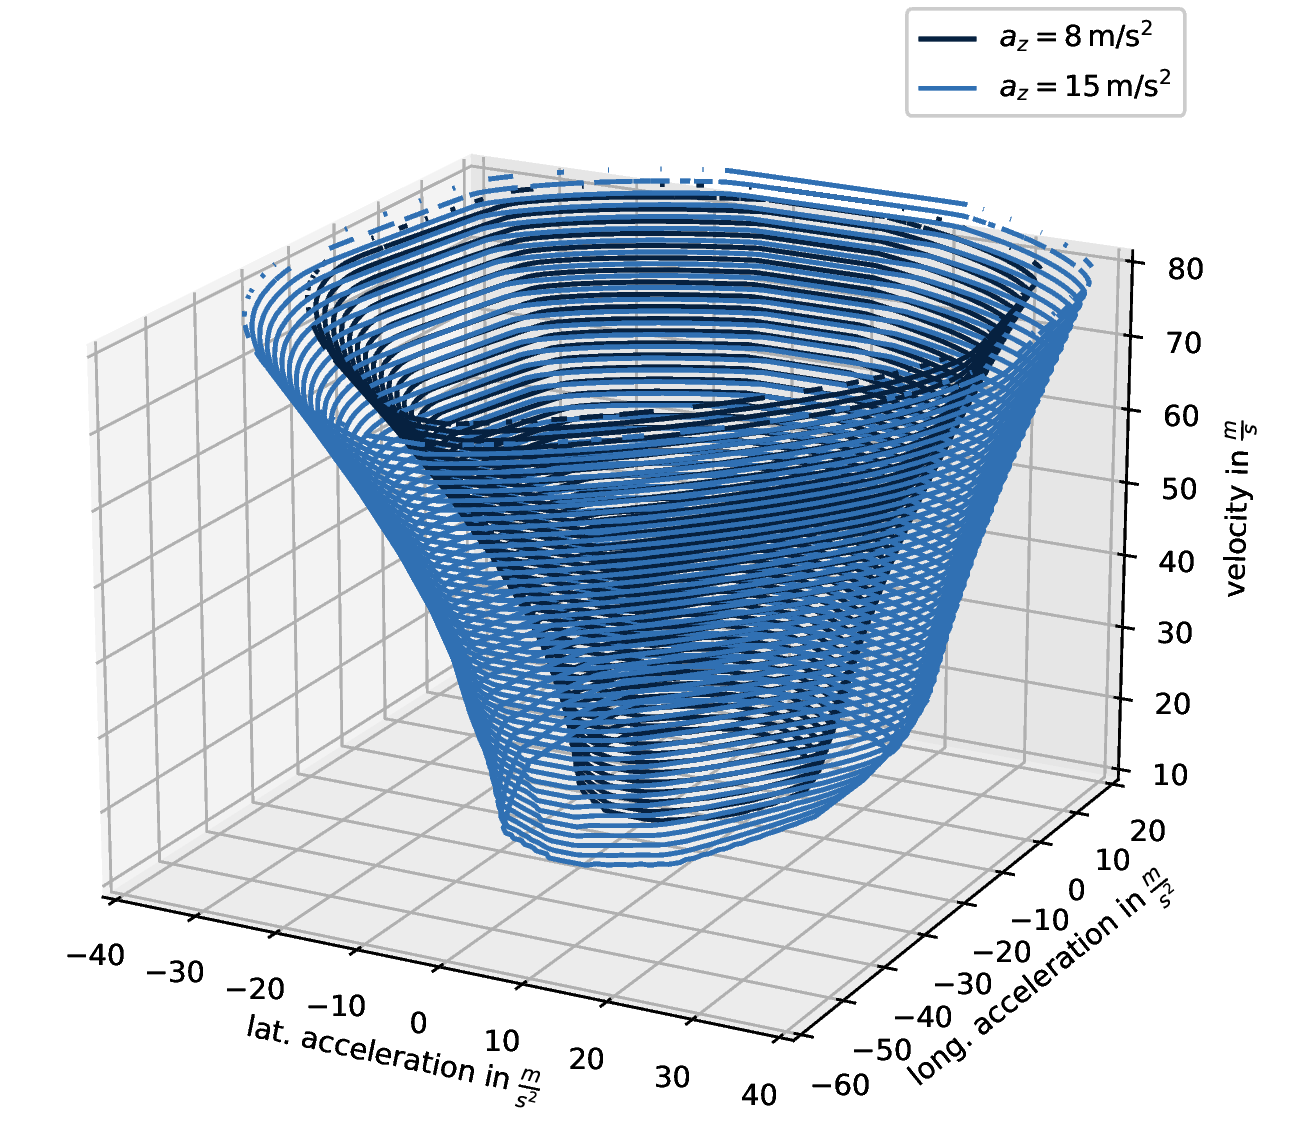
\includegraphics[width=0.6\textwidth]{figures/gggv_tornado.png}
    \end{center}
    \caption{Ενδεικτικό διάγραμμα επιδόσεων (\textit{GGV}) \cite{TUM_GGGVDiagrams}}
\label{fig:GGGV-Diagram-Sample}
\end{figure}

Στον αλγόριθμο προσομοίωσης γύρου, το προφίλ ταχύτητας $v(s)$ κατασκευάζεται με δύο διαδοχικές σαρώσεις κατά μήκος της
πίστας. Στην πρώτη, κατά τη φορά της πίστας, το όχημα επιταχύνεται σε κάθε σημείο με
το μέγιστο επιτρεπτό $a_x^+$, δίνοντας το προφίλ που περιορίζεται από την πρόσφυση κατά
την επιτάχυνση. Στη δεύτερη, με αντίστροφη φορά, το όχημα επιβραδύνει με το μέγιστο δυνατό
$|a_x^-|$, δίνοντας το προφίλ που περιορίζεται κατά την πέδηση προς την επόμενη στροφή.
Το τελικό $v(s)$ προκύπτει ως το κατά σημείο ελάχιστο των δύο σαρώσεων και ικανοποιεί
ταυτόχρονα το όριο πρόσφυσης στην κορυφή κάθε στροφής και την ικανότητα του οχήματος να
επιταχύνει και να επιβραδύνει εντός των ορίων του διαγράμματος \cite{Brayshaw2005}. Ο χρόνος
γύρου δίνεται τελικά από την ολοκλήρωση:

\begin{equation}
    T = \int_{0}^{L}\dfrac{ds}{v(s)}
    \label{eq:lapTimeIntegral}
\end{equation}

όπου $L$ το συνολικό μήκος της πίστας.\\[10pt]

Ο βασικός περιορισμός της προσέγγισης είναι ότι η τροχιά του οχήματος
θεωρείται δεδομένη, και ότι εξ ορισμού παραλείπονται μεταβατικά φαινόμενα με έντονη μη-μόνιμη
συμπεριφορά. Η σύγκριση με προσομοιωτές βέλτιστου ελέγχου καταγράφει μη-αμελητέες
αποκλίσεις υπέρ των μη-μόνιμων μεθόδων \cite{Perantoni2014}. Οι προσομοιωτές QSS ωστόσο, προτιμώνται λόγω του σημαντικά χαμηλότερου υπολογιστικού κόστους και τη δυνατότητα
άμεσης ενσωμάτωσης πρόσθετων μοντέλων -- όπως το θερμοδυναμικό μοντέλο ελαστικών της
παρούσας εργασίας -- μέσω κατάλληλης ενημέρωσης του διαγράμματος επιδόσεων GGV. Σημαντικότερα, η ανεξαρτησία τους από μοντέλο οδηγού τις καθιστά λιγότερο ευαίσθητες, αποτυπώνοντας μια ποσοτικοποίηση των μέγιστων επιδόσεων του οχήματος. 
